\documentclass[12pt,a4paper,twoside]{article}
\newcommand{\studentname}{Luigi Priano (1000002081)}
\title{Minimum Weight Vertex Cover using Tabu Search algorithm}

\newcommand{\tutor}{Mario Francesco Pavone, Vincenzo Cutello}

\newcommand{\reportdate}{10/02/2025}
\newcommand{\department}{D.M.I. Informatica LM-18 A.A. 2024/2025}

\usepackage[a4paper,left=32mm,right=32mm,bottom=32mm,top=32mm]{geometry}
\usepackage{listings}
\usepackage{color}
\usepackage{fancyhdr}
\usepackage{subfigure}
\usepackage{graphicx}
\usepackage{booktabs}
\usepackage[british]{babel}
\usepackage[square,comma,numbers,sort&compress]{natbib}
\usepackage{csvsimple}
\usepackage{graphicx}
\usepackage{pgfplotstable,filecontents}
\usepackage{gensymb}
\usepackage{array}
\usepackage{tabu}
\usepackage{multirow}
\usepackage{url}
\usepackage{hyperref}
\usepackage{amsmath}
\hypersetup{
    colorlinks=true,
    linkcolor=black,
    filecolor=magenta,      
    urlcolor=blue,
}

\urlstyle{same}
\usepackage{cleveref}
\pgfplotsset{compat=1.9}
\definecolor{bg}{RGB}{240,240,240}
\usepackage[utf8]{inputenc}
\usepackage[T1]{fontenc}
\usepackage{imakeidx}
\makeindex[columns=1, title=Indice]

\newcommand\MyBox[2]{
  \fbox{\lower0.75cm
    \vbox to 1.7cm{\vfil
      \hbox to 1.7cm{\hfil\parbox{1.4cm}{#1\\#2}\hfil}
      \vfil}%
  }%
}
\newcommand{\tpm}[1]{\colorbox{gray!25}{ \texttt{#1} }}
\renewcommand{\arraystretch}{1.5}


\begin{document}

\setlength{\parindent}{0em}
\setlength{\parskip}{0.5em}
\author{\studentname ~ \\ \\ Professori: \tutor.\\
\\
Dipartimento: \department}

\date{Data documento: \reportdate.}

\renewcommand\abstractname{Summary}

\pagestyle{fancy}
\fancyhead{}
\fancyhead[C]{\studentname~}
\fancyfoot{}
\fancyfoot[C]{\thepage}
\renewcommand{\headrulewidth}{0pt}
\renewcommand{\footrulewidth}{0pt}

\renewcommand\bibname{Riferimenti}
\renewcommand*\contentsname{Indice}
\renewcommand{\figurename}{Fig.}
\renewcommand{\tablename}{Tab.}

\begin{figure}[h!]
    \centering
    \maketitle
\end{figure}
\clearpage
\tableofcontents
\clearpage

\section{Minimum Weight Vertex Cover}
Il problema della Copertura dei Vertici a Peso Minimo (MWVC - Minimum Weight Vertex Cover) è un problema fondamentale nella teoria dei grafi con molte applicazioni pratiche, tra cui le comunicazioni wireless, la progettazione di circuiti e l'ottimizzazione dei flussi di rete. 
Una copertura di vertici di un grafo è un insieme di vertici tale che ogni arco del grafo ha almeno un estremo in questo insieme. Il problema MWVC estende il problema standard della copertura di vertici assegnando un peso positivo a ciascun vertice e cercando una copertura di vertici con il peso totale minimo. Il problema MWVC è NP-completo, il che significa che non esiste un algoritmo in tempo polinomiale noto per trovare la soluzione ottimale in tutti i casi.
\subsection{Definizione formale del MWVC}
Dato un grafo non direzionato $G = (V,E)$ con i pesi assegnati a ogni vertice, l'obiettivo del Minimum Weight Vertex Cover è quello di cercare tra tutti i possibili Vertex Cover $S \subset V$, l'insieme $S*$ la cui somma dei vertici è minima. \newline
La funzione obiettivo da minimizzare è: $\omega(S) = \sum_{v\in S}\omega(v)$ \newline Sapendo che: $\forall (v_i,v_j) \in E, v_i,v_j \in S, S \in V$
\newline
Una soluzione S è valida e si chiama Vertex Cover se ogni arco in G ha almeno un vertice in S. L'obiettivo della MWVC è quello di minimizzare la funzione obiettivo $\omega(S)$.
\section{Tabu Search algorithm}
L'algoritmo Tabu Search è una tecnica che guida una procedura di ricerca euristica locale per esplorare lo spazio delle soluzioni superando gli ottimi locali. Ad
ogni iterazione si considera un intorno dove sono state rimosse alcune soluzioni, definite tabù,
sulla base di una memoria del processo di ricerca effettuato fino a quella iterazione e le
soluzioni tabù non sono quindi raggiungibili all'iterazione successiva. Per “tecnica euristica” si
intende la ricerca di una buona soluzione, accettabile senza necessariamente raggiungere la
soluzione migliore assoluta, con un risparmio di risorse ed un risultato comunque soddisfacente. La Tabu Search si basa sulla premessa che la soluzione dei problemi deve incorporare una memoria adattabile e reagire durante l'esplorazione. L'uso di questa memoria contrasta con strutture "senza memoria" con quelle a "memoria rigida". L'esplorazione attiva della Tabu Search, sia in condizione deterministica che probabilistica, deriva dal presupposto che una cattiva scelta strategica può dare più informazioni rispetto a una buona scelta casuale. Il metodo di ricerca più conosciuto nel vicinato è quello di approssimare il valore minimo di una funzione f con valore reale in un insieme S detto metodo di discesa.
\subsection{Definizione formale}
Data una funzione $f(x)$ da ottimizzare su un insieme X, la Tabu Search inizia allo stesso modo ordinario della ricerca globale, procedendo iterativamente da un punto ad un altro fino a quando è soddisfatto un criterio di terminazione scelto. Ogni $x \in X$ ha associato un intorno di $N(x)\subset X$, e ogni soluzione x di N(x) è raggiungibile da x con un'operazione detta mossa. La ricerca va oltre l'insieme locale utilizzando una strategia di modifica di N(x) andando a sostituire il suo intorno N*(x). Se le soluzioni trovate non sono ottime vengono classificate come "tabù" e vengono rimosse dall'insieme N*(x). La gestione della memoria avviene tramite creazione di una o più tabù list, al loro interno si registrano gli attributi tabù-attivi e implicitamente o esplicitamente identificano il loro stato attuale. La durata di un attributo nel rimanere tabù-attivo si chiama tabù tenure e si misura in numero di iterazioni. Questa misura o livelli di tabù possono variare per i diversi tipi o combinazioni di attributi e possono anche variare nei diversi intervalli di tempo o fasi di ricerca. 
\subsection{Motivazioni della scelta dell'algoritmo}
La Tabu Search è stata preferita agli altri algoritmi presenti per l'esperimento a causa di diversi motivi. La preferenza rispetto al Branch and Bound è dovuta all'assenza delle informazioni iniziali sulle istanze, come il numero di nodi e la struttura degli archi. Nonostante si tratti di un metodo esatto, la mancanza di queste informazioni e la sua inefficienza nei grafi di grandi dimensioni ne hanno determinato l’esclusione. Rispetto agli algoritmi genetici, la Tabu Search ha il vantaggio di essere più mirata e di richiedere meno memoria. Questo perchè gli algoritmi genetici lavorano con una popolazione di soluzioni che comporta un costo computazionale elevato, mentre la Tabu Search opera su una singola soluzione alla volta evitando il problema della gestione di molteplici percorsi contemporaneamente. La Tabu Search, invece, si è dimostrata una scelta più adatta grazie alla sua velocità ed efficienza una volta implementata correttamente la memoria. A differenza del Branch and Bound non punta necessariamente a trovare la soluzione ottima, ma è in grado di individuare soluzioni di altà qualità in tempi molto brevi. Nel contesto dei MWVC, la soluzione sarà comunque ottimale, poiché i pesi dei vertici verranno analizzati e minimizzati. Di conseguenza, otterremo un metodo in grado di trovare l'ottimo in tempi brevi. Grazie alla lista Tabù questa ricerca permette di evitare di tornare su soluzioni già visitate, riducendo il rischio di cicli e migliorando l'efficacia della ricerca.
\clearpage
\section{Sviluppo dell'algoritmo}
L'algoritmo è stato sviluppato in due fasi differenti. La differenza principale tra i due script è l'ottimizzazione delle iterazioni e della memoria e la differente struttura di quest'ultima.
\subsection{Primo sviluppo}
Entrambi gli algoritmi sono stati sviluppati in Python (versione 3.11.5). Sono presenti diversi metodi, ognuno col proprio scopo, i principali vengono analizzati nei successivi paragrafi.
\subsubsection{Lettura del grafo}
\begin{verbatim}
Funzione LetturaGrafo(FileName)
    lines = FileName
    n = lines[0]
    weights = lines[1]
    matrix = lines[2:]
    Return n, weights, matrix
\end{verbatim}
Questo metodo legge un file e suddivide i dati in strutture appropriate. In particolare, weights è una lista che contiene i pesi associati ai vertici, mentre matrix è un array NumPy composto da liste, ciascuna rappresentante una riga della matrice di adiacenza. Quest'ultima descrive i collegamenti tra i vertici del grafo.
\subsubsection{Generazione dei vicini}
\begin{verbatim}
Funzione GeneraVicini(solution, n, matrix):
    neighbors = lista vuota
    soluzione_set = converti solution in un set
    # Rimozione di un nodo dalla soluzione
    Per ogni v in solution:
        new_solution = soluzione_set - {v}
        Se is_valid_cover(new_solution, matrix, n) allora
            neighbors add new_solution
    # Aggiunta di un nodo alla soluzione
    Per ogni v in {Tutti i nodi} - soluzione_set:
        new_solution = soluzione_set + {v}
        Se is_valid_cover(new_solution, matrix, n) allora
            neighbors add new_solution
    Return neighbors
\end{verbatim}
La funzione GeneraVicini genera tutte le possibili soluzioni vicine a solution rimuovendo o aggiungendo un nodo alla soluzione corrente. Solution viene gestita in un set per facilitarne le operazioni di aggiunta e rimozione dei nodi. L'obiettivo dei due cicli è quello di cercare le soluzioni possibili andando prima a rimuovere i nodi e poi aggiungendo quelli assenti, in modo tale da creare una lista valida di vicini.
\subsubsection{Tabu Search}
\begin{verbatim}
Funzione TabuSearch(n, weights, matrix, max_iter, 
tabu_tenure, max_no_improvement):
    # Inizializzazione
    current_solution = lista dei vertici
    best_solution, best_cost = current_solution, costo(current_solution)
    tabu_list = deque di lunghezza tabu_tenure
    no_improvement_count, visited_solution = 0, set vuoto
    # Tabu Search
    Per i in max_iter:
        neighbors = GeneraVicini(current_solution, n, matrix)
        Se neighbors è vuoto allora break
        best_neighbor, best_neighbor_cost = vuoto, infinito
        Per neighbor in neighbors:
            neighbor_tuple = sorted(neighbor)
            Se neighbor_tuple non è in tabu_list e visited_solution:
                cost = costo(neighbor)
                Se cost < best_neighbor_cost:
                    best_neighbor, best_neighbor_cost = neighbor, cost
        Se best_neighbor è vuoto:
            no_improvement_count += 1
        Altrimenti:
            current_solution = best_neighbor
            neighbor_tuple = sorted(best_neighbor)
            tabu_list + neighbor_tuple
            visited_solution + neighbor_tuple
            Se best_neighbor_cost < best_cost:
                best_solution, best_cost, no_improvement_count = 
                best_neighbor, best_neighbor_cost, 0
            Altrimenti:
                no_improvement_count += 1
        Se no_improvement_count >= max_no_improvement allora break
    Return best_solution, best_cost
\end{verbatim}
Lo pseudocodice soprastante implementa l'algoritmo della Tabu Search. Ad ogni iterazione genera le soluzioni vicine e seleziona la migliore non presente nella lista tabù o nella lista delle soluzioni già visitate. Se la soluzione trovata è migliore dell'attuale soluzione allora la sostituisce, altrimenti riprova a cercare una soluzione migliore fin quanto il valore di terminazione non raggiunge il limite di iterazioni. La lista degli elementi tabù impedisce di visitare soluzioni già visistate per evitare i cicli. L'algoritmo può terminare quando raggiunge il limite di iterazioni o quando non si migliora il valore attuale per un numero di iterazioni prestabilito.
\subsubsection{Risultati ottenuti}
Il primo sviluppo ha ottenuto ottimi risultati, trovando soluzioni ottimali in poche iterazioni. Tuttavia, il secondo sviluppo è stato introdotto per migliorarne l'efficienza, poiché il primo risultava troppo lento nel raggiungere l'ottimo globale, soprattutto con grafi di grandi dimensioni e numerosi archi. Questa lentezza è dovuta alle ripetute chiamate a determinate funzioni in ogni ciclo e a un uso non ottimizzato della memoria.
\subsection{Secondo sviluppo}
Il secondo sviluppo è stato implementato per ottimizzare il primo, concentrandosi sul miglioramento dell'uso della memoria e sulla riduzione delle chiamate superflue e dei passaggi ripetuti. Di seguito verranno analizzati i miglioramenti effettuati.
\subsubsection{Lettura del grafo}
Durante la lettura del grafo, il cambiamento principale riguarda l'uso di un array NumPy per i pesi dei nodi, al posto di una semplice lista. Questa modifica migliora le prestazioni, poiché gli array NumPy sono più efficienti e veloci rispetto alle liste standard di Python. Inoltre, gli array NumPy permettono di eseguire operazioni come somma e sottrazione senza la necessità di cicli espliciti, semplificando il codice e ottimizzando i calcoli.
\subsubsection{Generazione dei vicini}
All'interno di questa funzione sono stati apportati pochi ma significativi cambiamenti. La principale differenza riguarda l'uso delle operazioni sui set: nel primo codice veniva creata una copia del set in entrambi i cicli, mentre in questa versione le operazioni vengono eseguite direttamente sugli operatori dei set, senza la necessità di copiare l'intero set.\clearpage
\subsubsection{Tabu Search}
Nel metodo principale del codice sono state introdotte diverse ottimizzazioni. In primo luogo, è stato utilizzato frozenset al posto di tuple per rappresentare le soluzioni visitate e i vicini. I frozenset sono immutabili, più efficienti nelle operazioni di ricerca e possono essere usati come chiavi in strutture come set e deque, risolvendo anche il problema dei duplicati nelle soluzioni. Un'altra importante modifica riguarda l'introduzione di una heap per la gestione dei vicini, che permette di selezionare il miglior vicino con il costo più basso in modo più rapido ed efficiente, evitando il confronto manuale tra tutti i vicini. Queste modifiche migliorano la gestione delle soluzioni, riducono il numero di confronti e aumentano l'efficienza dell'algoritmo, rendendolo significativamente più performante.
\subsubsection{Altri metodi}
\begin{itemize}
    \item La funzione \texttt{is\_valid\_cover} è migliore della prima implementata perché sfrutta le operazioni vettoriali di numpy, che rendono il processo di verifica della copertura significativamente più veloce ed efficiente. Le operazioni bitwise consentono di eseguire il controllo in parallelo su intere righe e colonne della matrice, riducendo così la complessità computazionale e migliorando le prestazioni, soprattutto con grafi di grandi dimensioni. Inoltre, la funzione np.all() permette di verificare rapidamente se tutte le coperture sono soddisfatte in un unico passaggio;
    \item La funzione \texttt{evaluate\_solution} è migliore perché utilizza np.sum(), una funzione ottimizzata di numpy, per sommare gli elementi dell'array dei pesi. Questa versione è più efficiente in quanto esegue la somma direttamente sugli array senza passaggi aggiuntivi, ovvero, ciò che succedeva all'interno del primo sviluppo.
\end{itemize}
\subsubsection{Risultati ottenuti}
Le ottimizzazioni apportate hanno reso l'algoritmo più efficiente, garantendo prestazioni adeguate al carico di lavoro. Nonostante il numero di iterazioni rimanga invariato per i diversi grafi, l'algoritmo fornisce comunque la soluzione ottima in tempi ridotti rispetto al primo sviluppo.
\section{Risultati finali}
Di seguito sono riportati i risultati ottenuti per tutte le istanze dell'esperimento. Per ragioni di efficienza, è stato utilizzato solo il secondo sviluppo, avendo verificato su grafi campione che il primo sviluppo produce gli stessi risultati. Le istanze sono presenti all'interno dei file txt così formati:
\begin{itemize}
    \item Prima riga: numero di vertici;
    \item Seconda riga: pesi dei vertici;
    \item Dalla terza riga: matrice degli archi grande N x N dove N è il numero dei vertici. Sono presenti 0 quando non è presente un arco e 1 quando l'arco è presente.
\end{itemize}
\subsection{Grafo 800 Vertici, 10000 Archi}
Questo è il grafo più complesso tra le istanze analizzate, con 800 vertici e 10.000 archi, risultando significativamente più impegnativo rispetto agli altri grafi dell'esperimento. Entrambi gli algoritmi hanno individuato la soluzione ottima, con un costo di 46.393 e un totale di 113 iterazioni, completate in soli 128.0274 secondi (circa 2 minuti e 8 secondi) utilizzando il secondo sviluppo. Nella figura di seguito è mostrato il grafo in tutta la sua complessità. I nodi in blu sono quelli non presenti all'interno della MWVC, mentre quelli in rosso sono presenti.
\begin{figure}[!h]
    \centering
    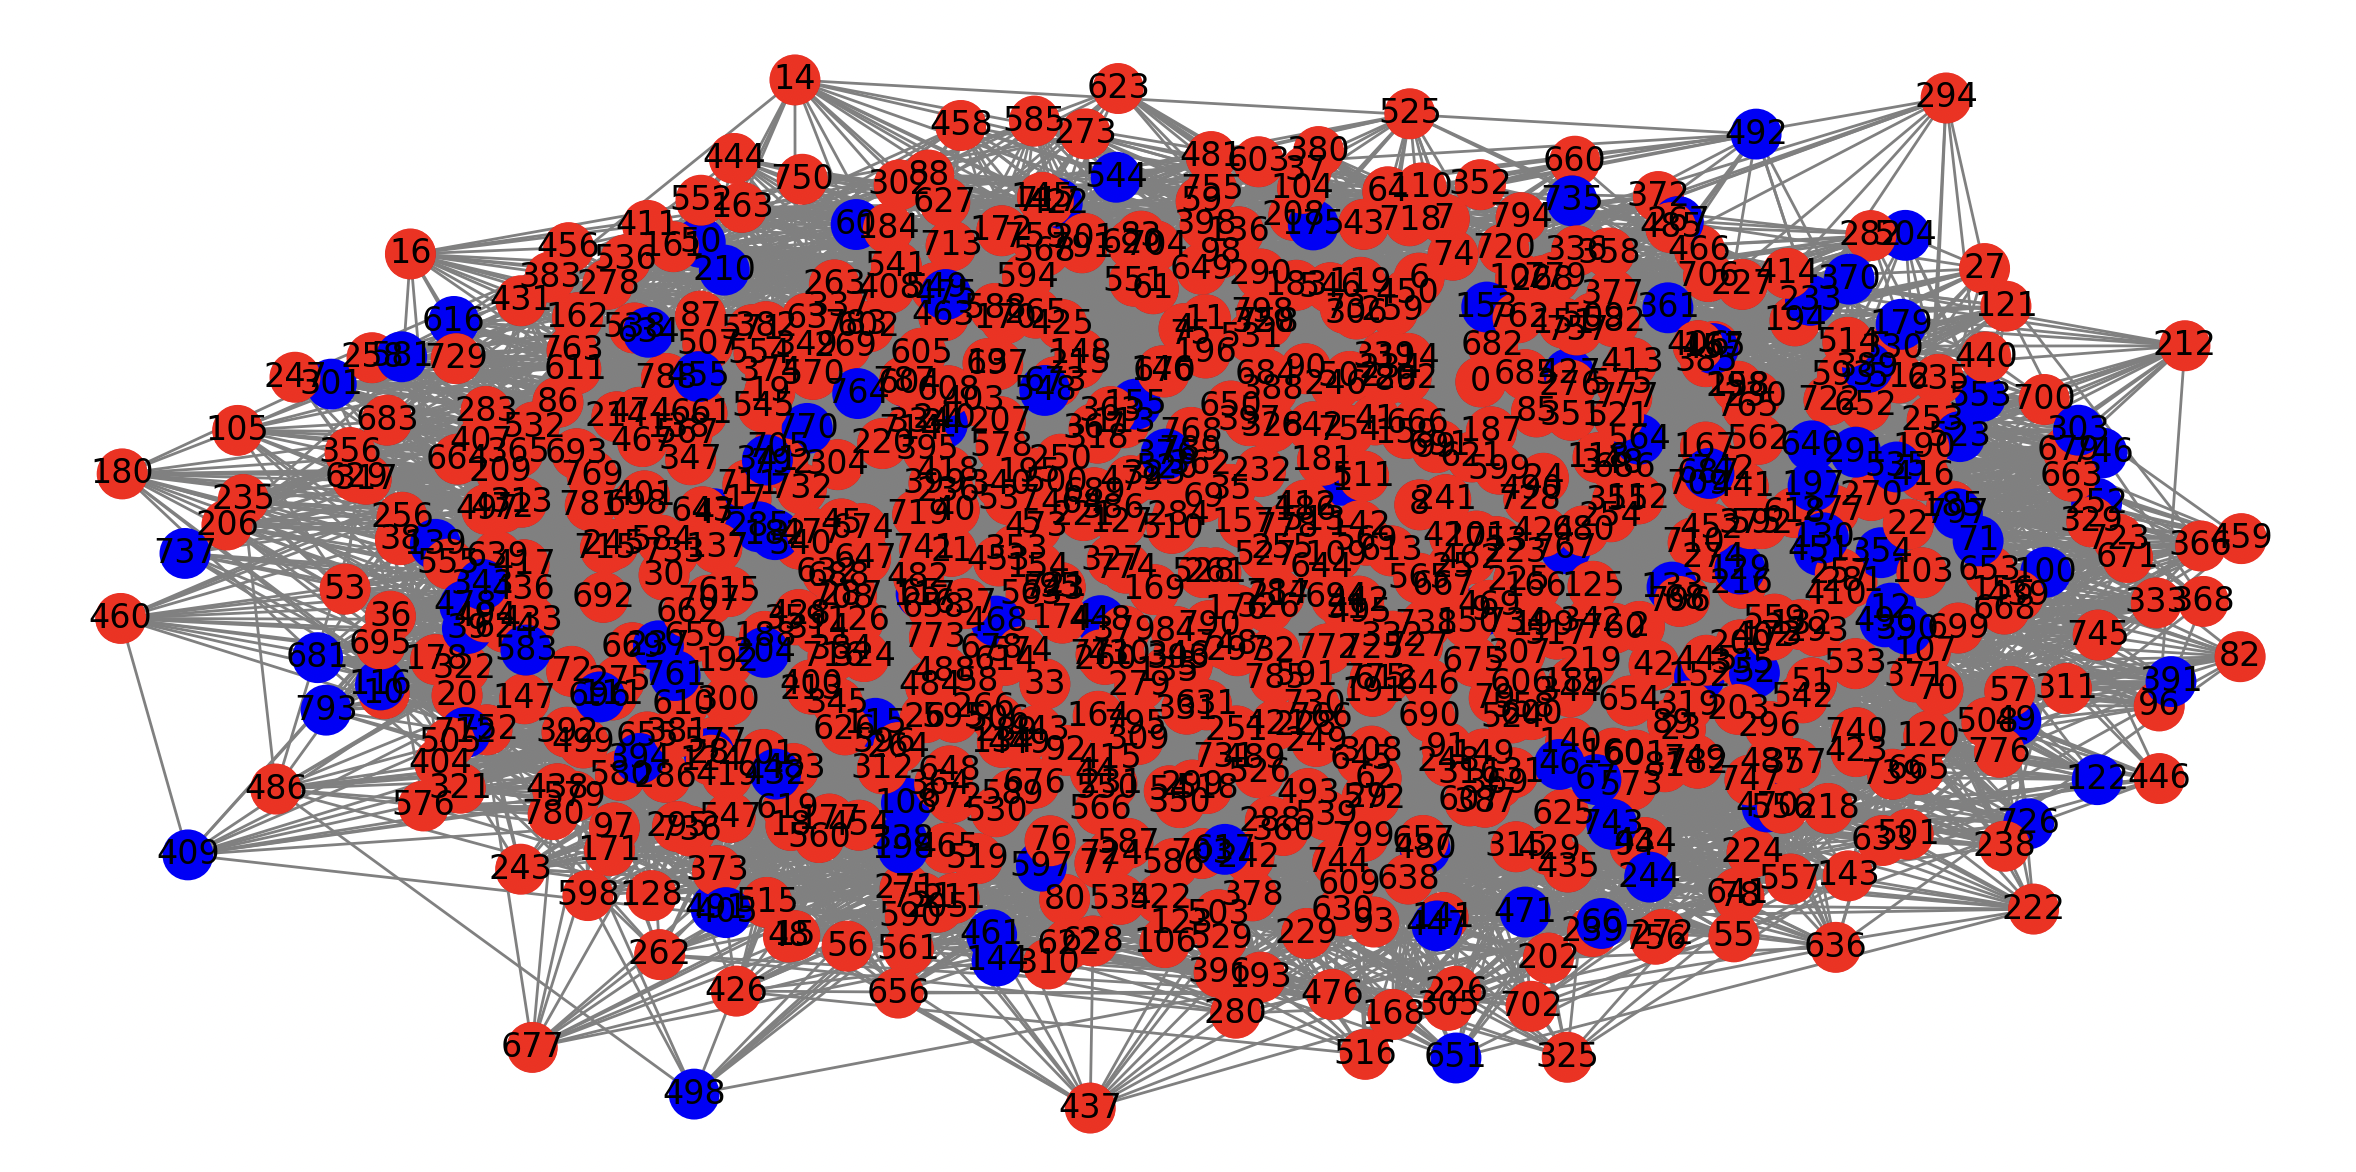
\includegraphics[width=0.8\linewidth]{Graph800-10000.png}
    \caption{Grafo vc\_800\_10000}
    \label{fig:enter-label}
\end{figure}
\newline
La soluzione del vertex cover è la seguente:
\begin{figure}[!h]
    \centering
    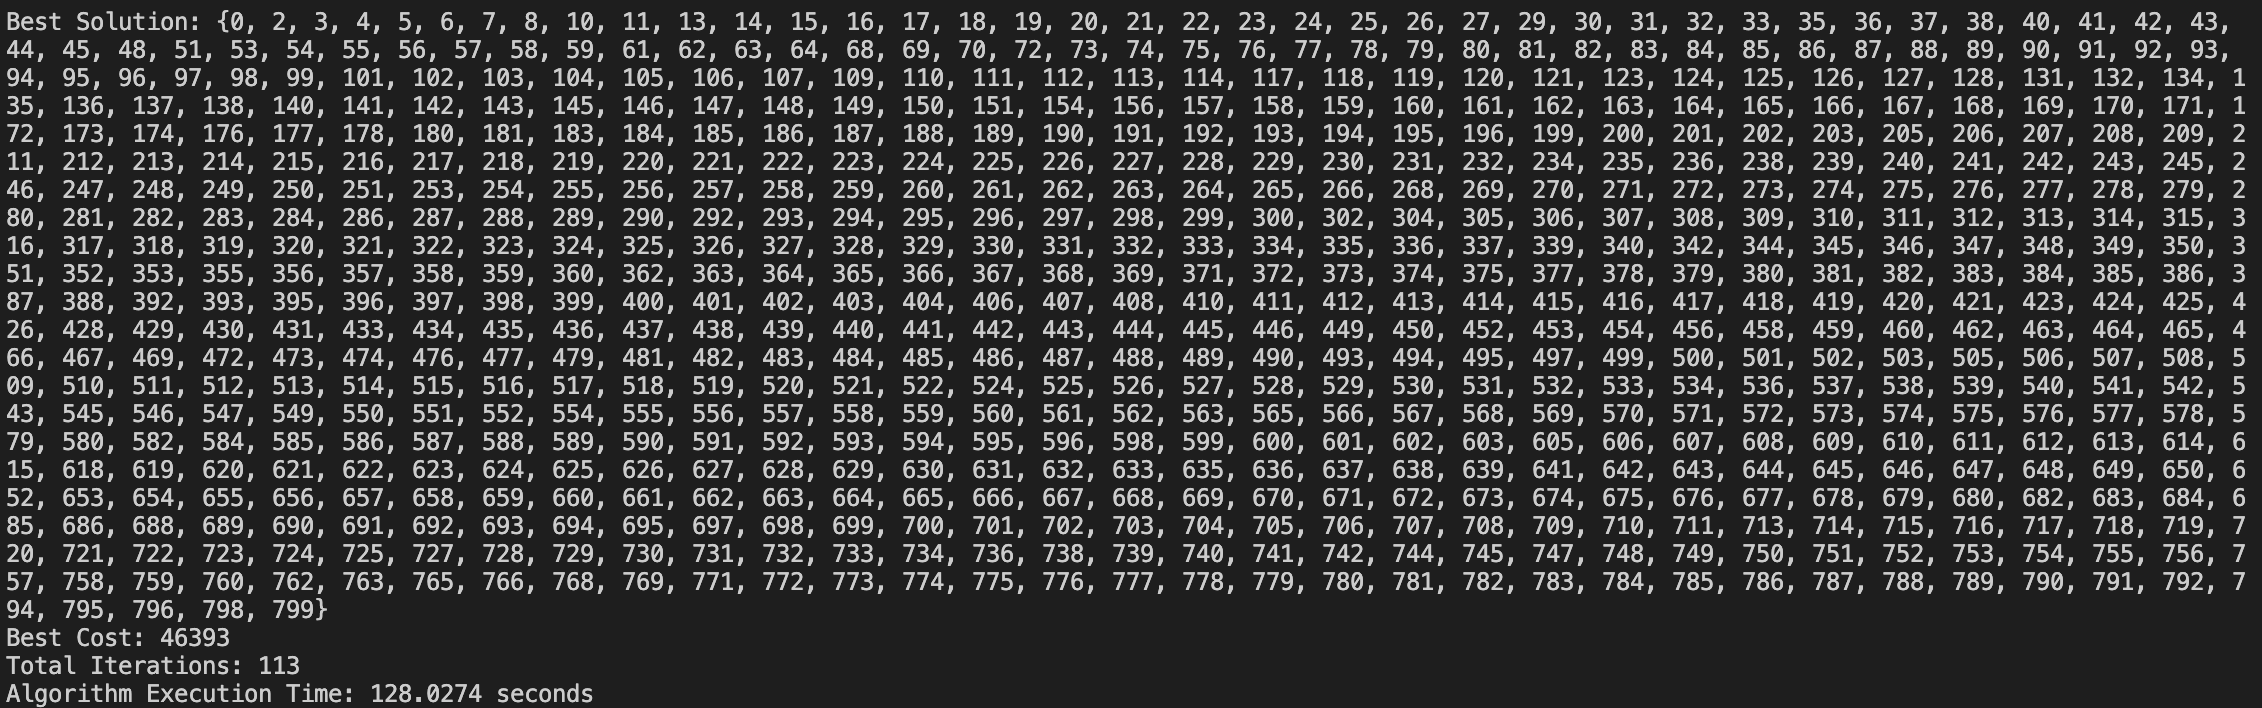
\includegraphics[width=0.8\linewidth]{BestSolution800-10000.png}
\end{figure}
\clearpage
\subsection{Altri grafi}

\begin{figure}[!h]
    \centering
    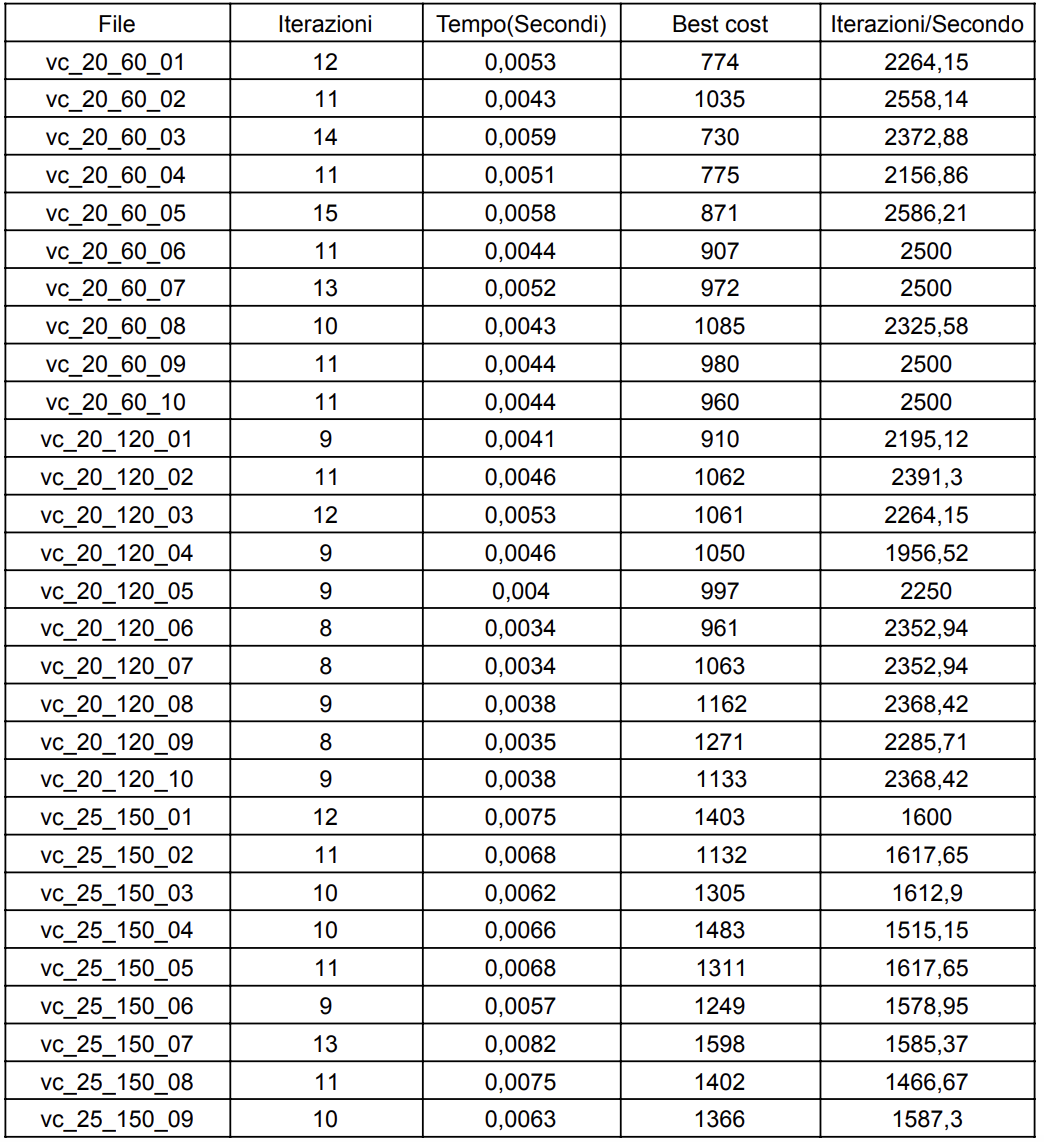
\includegraphics[width=0.56\linewidth]{Graph1.png}
    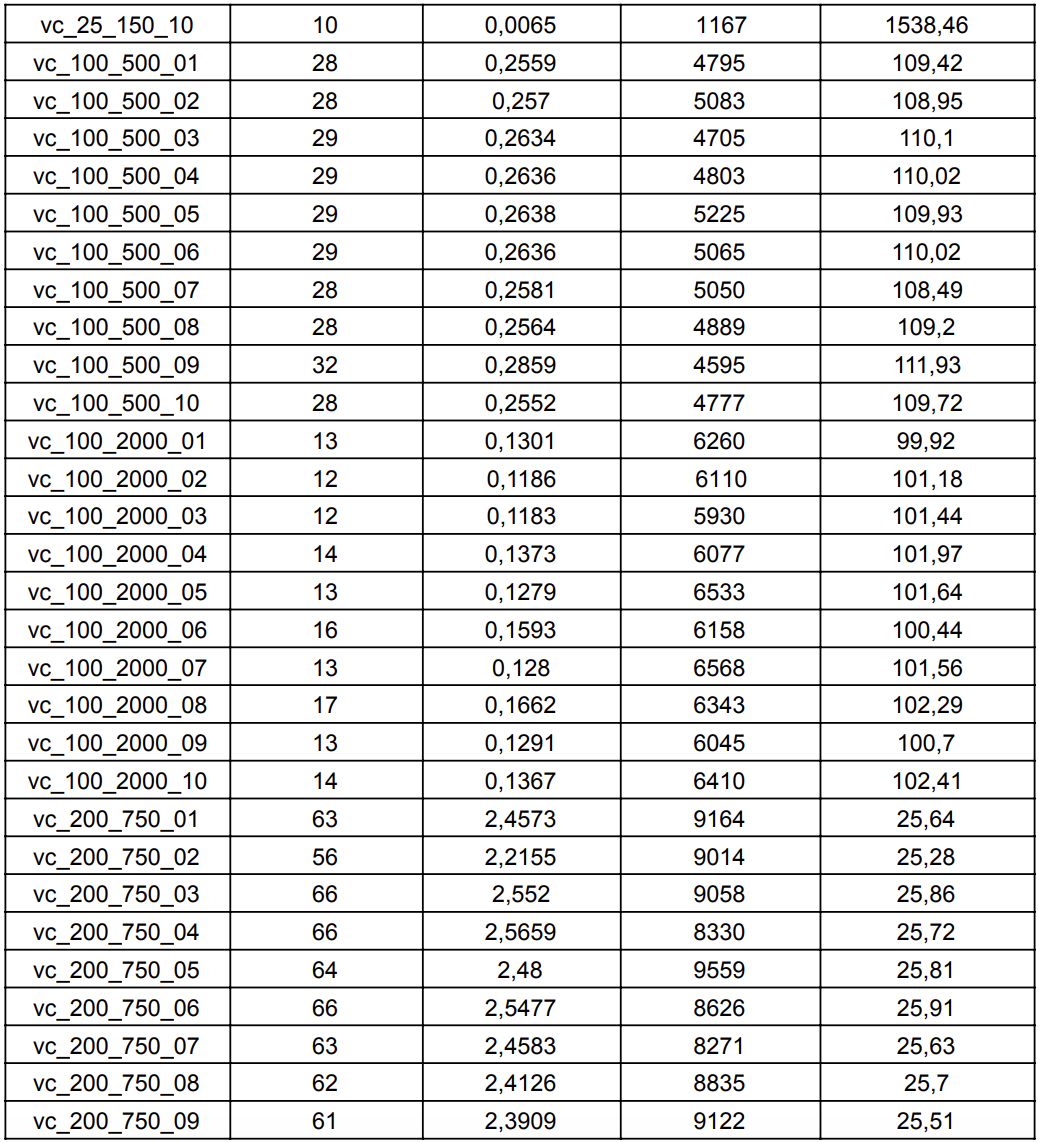
\includegraphics[width=0.56\linewidth]{Graph2.png}
    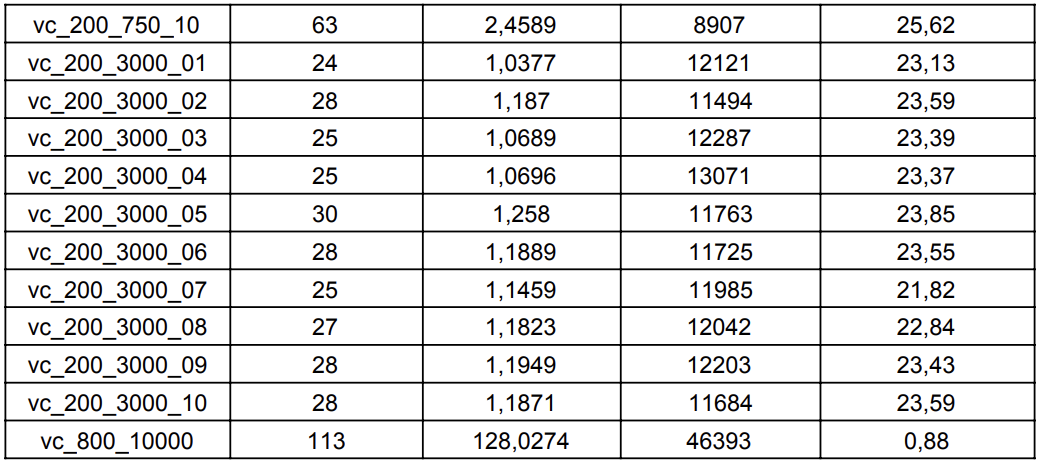
\includegraphics[width=0.56\linewidth]{Graph3.png}
\end{figure}
\subsection{Differenza di prestazione tra i due sviluppi}
In questo paragrafo saranno analizzate le differenze di prestazioni tra i due sviluppi, considerando tre grafi di diversa complessità: uno semplice, uno di media difficoltà e uno complesso.
\begin{enumerate}
    \item vc\_20\_60\_01: questo grafo è formato da 20 nodi pesati e 60 archi totali:
    \begin{itemize}
        \item Primo sviluppo: 12 iterazioni in 0.0130 secondi;
        \item Secondo sviluppo: 12 iterazioni in 0.0050 secondi.
    \end{itemize}
    \item vc\_100\_500\_01: questo grafo è formato da 100 nodi pesati e 500 archi totali:
    \begin{itemize}
        \item Primo sviluppo: 28 iterazioni in 3.0399 secondi;
        \item Secondo sviluppo: 28 iterazioni in 0.2552 secondi.
    \end{itemize}
    \item vc\_200\_3000\_01: questo grafo è formato da 200 nodi pesati e 3000 archi totali:
    \begin{itemize}
        \item Primo sviluppo: 24 iterazioni in 25.1012 secondi;
        \item Secondo sviluppo: 24 iterazioni in 1.0292 secondi.
    \end{itemize}
\end{enumerate}
Questi test dimostrano chiaramente che, nei casi più semplici, il secondo sviluppo è 2.6 volte più veloce del primo. Con l'aumentare della complessità, il divario si amplifica: nel caso di media difficoltà, il secondo sviluppo risulta 11.91 volte più rapido, mentre nel grafo più complesso la velocità aumenta fino a 24.4 volte. Questo risultato conferma l'efficacia dell'ottimizzazione effettuata, che ha permesso un significativo miglioramento delle prestazioni dell'algoritmo lasciando inalterata la sua efficacia.
\subsection{Differenza nell'uso dell'elemento tabu\_tenure}
Per completezza, è stata effettuata una prova con diversi valori di \texttt{tabu\_tenure}. Durante tutti gli esperimenti, il parametro è stato impostato a 8, un valore considerato ottimale in quanto bilancia la possibilità di esplorare soluzioni ottime evitando al contempo di creare una lista tabù troppo grande. È stato anche testato un valore di \texttt{tabu\_tenure} pari a 2, riscontrando un lieve rallentamento nei grafi con più nodi, con un incremento di circa 10 secondi sull'intera esecuzione. Aumentando ulteriormente il \texttt{tabu\_tenure} a 20, si è registrato un rallentamento di circa 3 secondi. Tuttavia, in entrambi i casi, il miglior valore è stato ottenuto con lo stesso numero di iterazioni di quando si utilizza il valore di 8.
\section{Conclusioni}
Il progetto ha analizzato due algoritmi basati su Tabu Search per affrontare il problema del Minimum Weight Vertex Cover (MWVC), ottenendo risultati notevoli. Il primo algoritmo, sebbene più lento, ha dimostrato l'efficacia della Tabu Search nel trovare la soluzione ottima in poche iterazioni, anche se il tempo di esecuzione può rappresentare un limite significativo nei grafi di grandi dimensioni. Il secondo algoritmo, ottimizzato per migliorare le prestazioni, ha ridotto drasticamente i tempi di calcolo, mantenendo comunque la capacità di raggiungere il valore ottimo in poche iterazioni. Quest'ottimizzazione si è rivelata particolarmente vantaggiosa per grafi di dimensioni elevate. Durante l'esperimento, è emerso che, nei grafi con pochi nodi, la differenza tra i due algoritmi è netta, ma anche il primo algoritmo ha mostrato ottime prestazioni, con tempi di esecuzione nell'ordine dei centesimi di secondo. Tuttavia, al crescere del numero di nodi, la differenza diventa più evidente, con l'algoritmo ottimizzato che garantisce prestazioni notevolmente migliori, riducendo il tempo di risposta da secondi a frazioni di secondo. In particolare, l'algoritmo ottimizzato potrebbe essere impiegato in applicazioni quasi in tempo reale per grafi con meno di 100 vertici, mentre per grafi superiori a 200 vertici si osserva un aumento del ritardo, con un tempo di risposta minimo di circa 2 secondi.
Questi risultati evidenziano come la scelta dell'algoritmo Tabu Search sia una soluzione particolarmente efficace per il problema del MWVC, rivelandosi una scelta vincente per l'esecuzione dell'esperimento.
\section{Riferimenti}
\begin{enumerate}
    \item[{[1]}] \label{1} \href{https://en.wikipedia.org/wiki/Vertex_cover}{Vertex Cover (2024)}
    \item[{[2]}] \label{2} \href{https://thesis.unipd.it/retrieve/72861d68-61b5-45f6-94af-a86b25726440/tesi_Tabu_Search_21.2.2112.pdf}{L’algoritmo “Tabu Search” per l’ottimizzazione, teoria ed applicazioni (2012)}
    \item[{[3]}] \label{3} \href{https://github.com/Luigi018/IA-Project}{IA-Project, Luigi Priano (2025)}
\end{enumerate}
\printindex
\end{document}
